\chapter{Experimental Setup and Evaluation}
\begin{comment}

    Experimental Setup and Evaluation

- Goal of Experiment
- Methods and actual tools used
- Experimental Setup in detail
- Experimental procedure
- Presentation of experimental results

update to overleaf since git is not working!

\end{comment}

This chapter will go over the experimental aspect of this work including the tools and equipment used to implement the algorithms. The setup of the experiments and the testing done on each algorithm and the process of developing these algorithms. The benchmarking results for the two discovery algorithms will be discussed.

We will also present the experimental results for the two algorithms as a proof of concept for the algorithms as presented in the previous chapter.



\section{Equipment and Modeling}
The FESTO water management system was designed for educational purposes in automation. For this work it was equipped with two sensors and three actuators. All of the capabilities of these sensors and actuators are exposed as web resources on three NodeMCU ESP8266 microcontrollers following the Web of Things architecture. Below is the mapping of the microcontrollers to their actuators. In addition to each of the capabilities of their mapped actuators each microcontroller exposes the resources \texttt{/urdfl} and \texttt{/urdfq}, allowing the device to load and query RDF data respectively. In this case the NodeMCU 3 has been mapped multiple devices.

\vspace{1cm}
\begin{figure}[ht]
\centering
\begin{tabular}{l | l}
  water level sensor (LUT400) & NodeMCU 1 \\
  flow sensor (Sitrans F M Mag 6000) & NodeMCU 2 \\
  on/off valve & NodeMCU 3 \\
  pump on/off switch & NodeMCU 3 \\
  water heater on/off switch & NodeMCU 3 \\
\end{tabular}
  \caption{Mappings of Servients to Sensors \& Actuators}
  \label{table:mappings}
\end{figure}

The FESTO unit was originally built as a pedagogical tool to help engineers learn about automation. Here it serves as a minimal viable model of a water reclamation facility. Because the benchmarks only required the semantic data, it was unnecessary to use the FESTO unit while conducting the tests. Instead each experiment was conducted on a with the three NodeMCUs connected to a PC.

\begin{figure}[th]
\centering
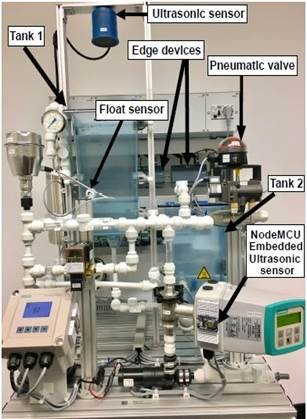
\includegraphics[width=.7\textwidth]{Figures/festoDemonstrator.jpg}
\caption{The FESTO Demonstrator}
\label{fig:festoDem}
\end{figure}



\section{Tools Used}
This section will discuss the hardware and software required to implement and test the algorithms.

\subsection{Apache Jena}

Apache Jena is a Java framework used to build Semantic Web applications. It entails various APIs, which work together to process RDF, OWL, and SPARQL. The centralized discovery algorithm required Apache Jena in order to manipulate blank nodes.

There are several modules within Apache Jena, in this paper the most  used was the Core RDF API. In the Core RDF API RDF Graphs can be represented by the data structure \texttt{Model}, which is composed of \texttt{Statements} or may be implemented in the simpler and more limited Java API \texttt{Graph}. \texttt{Statements} entailing one subject, predicate, and object represent a \textit{triple} and are immutable in Jena. This means triple had to be altered when piecing together connected graphs, such as in the \texttt{GraphLean} algorithm, the new \texttt{Statement}s had to be created with the updated information and the old Statement could then be removed from the \texttt{Model} and the new one appended. This process was not included in the benchmarking times, since took place on aa PC and the primary interest was the amount of time message passing required. \cite{Jena.24.10.2017}

\subsection{ESP8266}

The ESP8266 is an inexpensive Wi-Fi capable system on a chip (SoC) manufactured by the Chinese company Espressif. It fully supports the TCP/IP stack and 802.11 b/g/n/d/e/i/k/r. The ESP8266 has a small amount of flash memory available--only about 512 kB, though this can be upgraded to 4 MB. The algorithms created in this work were tested using the NodeMCU version of this chip, which includes a special firmware for IoT development. \cite{Zeroday.2017}


This microcontroller is unquestionably rugged: it has an operating temperature range spanning from -40\textdegree{}C to 125\textdegree{}C and is therefore suitable for a wide spectrum of applications. It can be used for home applications, including home automation: monitoring home appliances, monitoring the energy output of photovoltaic cells, managing lights and outlets, baby monitors, etc. It's wide operating temperature range also makes it an appropriate choice in industrial wireless control networks and sensor networks. \cite{espDatasheet} Additionally the ESP8266 has a modest price and is available starting at 5 EUR if purchased individually, with bulk pricing hovering around 1 EUR per unit.

There are several versions of firmware publicly available for the ESP8266, Siemens created a proprietary version based off of the NodeMCU firmware. The Siemens version of the NodeMCU firmware allows the NodeMCUs to expose their ability to have semantic data queried, using the \texttt{/urdfq} resource, and loaded using the  \texttt{/urdfl} resource. Without these two Web resources the client would not be able to access the semantic data on the NodeMCUs. 

Another key feature of the NodeMCU firmware is the integration of embedded Lua (eLua) \cite{Zeroday.2017}, which entails the same features as the desktop version plus additional features useful for embedded developers. Like Lua, eLua is able to run on nearly every platform, because it was implemented in ANSI C. \cite{Marinescu.} 

Lua is an extensible language, meaning it can integrate functions, which cannot (or should not) be directly written in Lua. This works using the C API, which allows code written in C to interact with Lua. The C API is also available in eLua. The combination of the simplicity and high-level abstraction of a scripting language with the portability and light-weight implementation in C \cite{luaHandbook}, means eLua is powerful tool for embedded developers. This work used Lua in the distributed discovery algorithm.
% https://nodemcu.readthedocs.io/en/master/en/upload/ TODO: continue



\change{removed other picture of NodeMCU, add your own picture of ESP8266, others are copyrighted}

\subsection{ESPlorer}
ESPlorer is an IDE used by ESP8266 developers. It can run on Windows, Linux, MacOS, and Solaris and it provides tools for working in Lua for the NodeMCU and MicroPython. For benchmarking it was run in a virtual machine running Ubuntu 16.04.

\begin{figure}[h]
\centering
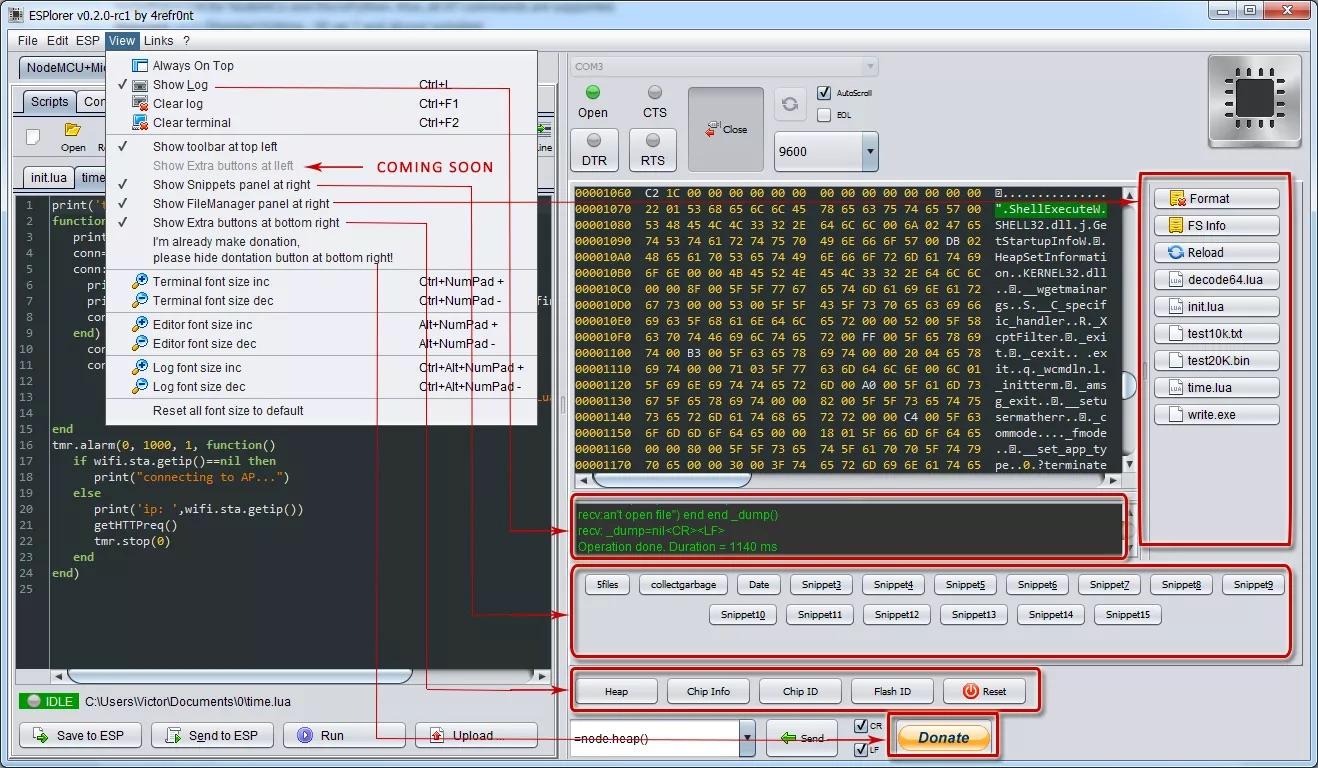
\includegraphics[width=\textwidth]{Figures/ESPlorer.jpg}
\caption{The ESPlorer interface. Image is from the NodeMCU documentation\cite{Zeroday.2017}}
\end{figure}

Code is written in the buffer on the left, while the right buffer shows the current status and connection to the NodeMCU. Connecting to the NodeMCU is simple: after plugging the NodeMCU in, users hit the refresh button in the upper-right corner, then select the COM port, and finally the baud rate.

After a connection to the NodeMCU has been established, code can be simply added and removed from the NodeMCU using buttons in the lower left side of the IDE.

\section{Experimental Procedure}
This section will outline the implementation details for the algorithm implementations in this work, specifically how they were implemented, how they were tested, and how they were benchmarked. In each subsection, the results of the tests/benchmarks will be discussed.


\subsection{The REDD Algorithm}

The REDD algorithm was vital to the centralized discovery. Since the REDD Algorithm as presented by Esposito et al. was incorrect, we wanted to ensure what we contributed delivered what was intended. Our version of the REDD algorithm was verified by unit testing with JUnit. This includes checking that the queries that were created were created from the models were converted correctly. This was especially important when forming queries containing blank nodes.


Other JUnit tests were created to test the correctness of the algorithms using trivial dummy RDF graphs. This ensured that the resultant blank RDF node pairs computed by the algorithm were in fact correct. Unit tests checked that the blank node connected graphs were created correctly and that the redundant blank node pairs were correct.

Since we had the pseudocode from Esposito (Figure \ref{fig:EspositoListing}), this was used as a framework for our implementation. First the simpler algorithms were implemented, like the \texttt{ExecuteQuery} and the \texttt{BuildConnGraphs} functions. This was estimated to take about two weeks--but ended up requiring more than three months, since the original paper did not contain adequate information to recreate the algorithm and contained definitions from the W3C recommendations used without any further explanation. Other than that the article was vague and even incorrect as submitted, according to one of the paper's co-authors.

Lastly a data type for the connected graphs (\texttt{ConnectedGraph}) was created, as well as a data type for the pairs of \texttt{RDFNode}s, called \texttt{RDFNodePair}.

\begin{figure}[h]
\centering
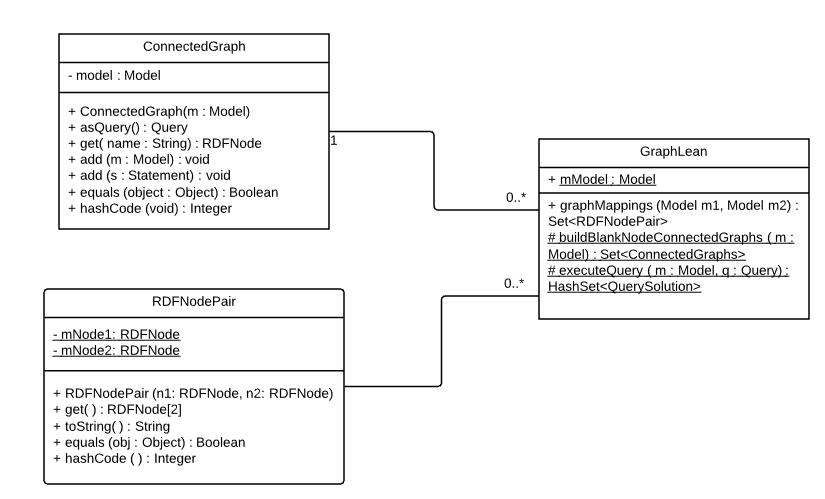
\includegraphics[width=\textwidth]{Figures/REDDuml.png}
\caption{The UML diagram of the implemented REDD Algorithm.}
\end{figure}

We started by implementing the the pseudocode as it was likely intended to be implemented: one graph was processed and searched for redundant subgraphs. As discrepancies came up in the implementation, we reached out to the author, but since the paper was so old (2005), the author no longer had any code and expressed that she neither had the "time, nor the interest" in discussing the algorithm further. So left to our own devices, we rebuilt the algorithm, as we thought was intended and verified using unit testing.

For the tests we created sample data using the Turtle format; like the below, which contains 6 triples and 3 connected subgraphs. When the more simplistic graphs passed tests, then we repeated the tests on the functions using the actual semantic data from each device. We then tested the \texttt{buildBlankNodeConnectedGraphs} function, by checking that number of blank node connected graphs were correct. This test is shown in listing \ref{blankNodeJUNIT}.

\begin{lstlisting}[caption={Some sample data that we created for unit testing, written in Turtle.}, frame=single]
@prefix person: <http://example.com/person/fake/>

person:adam		<p>            _:b3 .
_:b3			<p>		_:b4 .
person:adam		<p>		_:b1 .
_:b1			<p>		_:b2 .
_:b2		        <p>	person:bertold .
person:bertold  	<p>		_:b5 .
\end{lstlisting}
\vspace{.5cm}

Listing \ref{blankNodeJUNIT} shows the basic setup of a JUnit Test. The test is marked with a \texttt{@Test} tag before the function declaration. Then an instance of the class to be tested is created. A function was implemented to convert sample Turtle RDF graphs into Jena Models and then the function \texttt{buildBlankNodeConnectedGraphs} was run using the sample model. The actual test is in the last line, where \texttt{assertEquals} checks that the number of connected graphs created by the method is indeed three.

\begin{lstlisting}[language=JAVA, caption={A trivial test, that checks the correct number of connected graphs in a sample graph is correct for the sample data, in this case sample.ttl contains 3 connected subgraphs.}, label={blankNodeJUNIT}, tabsize=2, breaklines=true, frame=single]
@Test
public void buildConnGraphsTest() {
  GraphLean tester = new GraphLean();

  Model m = createSampleModel("sample.ttl");
  Collection<ConnectedGraph> graphs = tester.buildBlankNodeConnectedGraphs(m);
  assertEquals("Num connected Graphs is correct", 3, tester.buildBlankNodeConnectedGraphs(m).size());
}
\end{lstlisting}
\vspace{.5cm}

This test was run multiple times using different dummy data and each time it passed, so after that the next methods were implemented. Since the foundation of the REDD algorithm worked--namely the creating of blank node connected graphs from a given model, we then moved on to checking if graphs containing blank nodes could be queried without failure.

The following turns a model that does not contain blank nodes into a query, which is run against a graph which does contain blank nodes. With this particular sample data, no result was expected. This test was implemented in several variations: e.g. with the queried graph containing no blank nodes and the query model containing blank nodes. And all variations thereof. Each iteration of the test passed--so it seemed that that was not a problem. Finally, the last function in the REDD algorithm could be implemented.


\begin{lstlisting}[language=JAVA, caption={This test checks if a model containing blank nodes can be queried without returning an error.}, tabsize=2, breaklines=true, frame=single]
@Test
public void blankModelExecutionTest() {
	GraphLean tester = new GraphLean();
	// m contains no blank nodes
	Model m = createSampleModel("sample4.ttl");
	ConnectedGraph connGraph = new ConnectedGraph(m);
	// mQueried contains blank nodes
	Model mQueried = createSampleModel("sample5.ttl");
	Query q = connGraph.asQuery();
	HashSet<QuerySolution> solutions = tester.executeQuery(mQueried, q);
     // no solutions expected
	assertTrue("No solutions found", solutions.size() == 0);
}
\end{lstlisting}
\vspace{.5cm}

Once the REDD algorithm was implemented as it was \textit{most likely} intended in Espoisto's paper, we changed the graph mappings function, to run queries between two graphs: $G_1$ and $G_2$. Finally, this algorithm could be used to update graphs in the centralized discovery algorithm. Each step of the way we ran tests to ensure the algorithm was still functioning correctly, as seen above.

The final test took all three NodeMCUs and created the lean subgraph in the network, i.e. the \textit{core} graph, that all of the NodeMCUs should have. Since this test seen in \ref{lst:coreJUNIT} and all others came back correctly, we continued on to implement the centralized discovery algorithm. The core graph is the same graph seen in figure \ref{fig:festoUnion}--finally this is the graph that each node should have by the end of the centralized discovery algorithm.

\begin{lstlisting}[language=java, caption={The final test, which checked that the semantic data was being connected, as previously expected.}, label={lst:coreJUNIT}, tabsize=2, breaklines=true, frame=single]
@Test
public void findRedundanciesInGraphsTest() {
  GraphLean tester = new GraphLean();

  Model actuators = createSampleModel("actuators.ttl");
  Model lut400 = createSampleModel("lut400.ttl");
  Model pmag = createSampleModel("pmag.ttl");

  Model merged = ModelFactory.createDefaultModel();

  Set<RDFNodePair> redundancies;

  redundancies = tester.graphMappings(actuators, pmag);
  redundancies.addAll(tester.graphMappings(pmag, lut400));
  redundancies.addAll(tester.graphMappings(actuators, lut400));

  merged.add(actuators);
  merged.add(pmag);
  merged.add(lut400);

  List<Statement> toRemove = new ArrayList<>();
  StmtIterator it = merged.listStatements();
  while (it.hasNext()) {
    Statement st = it.next();
    for (RDFNodePair p : redundancies) {
      RDFNode[] array = p.get();
      // take blank node in pair
      RDFNode n = array[0].isAnon() ? array[0] : array[1];
      if (n.equals(st.getSubject()) || n.equals(st.getObject())) {
        toRemove.add(st);
      }
    }
  }
  merged.remove(toRemove);

  Model systemcore = createSampleModel("system-core.ttl");

  assertTrue("Merged Graphs should equal syscore", merged.isIsomorphicWith(systemcore));
}
\end{lstlisting}



\subsection{The Centralized Discovery}

The set-up for the centralized discovery was quite simple: the three NodeMCUs are connected to a PC, which acts as the client.

Each iteration of the centralized discovery can be broken down into two steps: (1) the semantic graphs are combined (2) the resultant lean graphs are sent to the respective servient. Benchmarks measured the time it took for the graphs to be processed with the REDD algorithm and the amount of time it took for the graphs to be sent to the servients, the latter being especially relevant for this work. The former is largely dependent on hardware capability and is therefore not particularly noteworthy--all that matters here is that it functioned, which was proven using JUnit tests.

The centralized algorithm was implemented by using psuedocode and implementing the code, again using Apache Jena. The implementation of the centralized discovery was straight forward and did not require much testing. The only unit testing that was done checked if all three devices had the same core graph when the discovery algorithm finished running. When this test passed, the benchmarks were run.

\change{add uml diagram, love}


\change{add activity diagram, maybe in theory part?}

The benchmarks seen in listing \ref{lst:centralizedBenchmark} were run using a normal PC connected to the three microcontrollers via USB. The benchmark was run, so that each iteration of the centralized discovery would pause and could be continued manually. As stated above, only the message times were recorded, since they were the main interest.

In the benchmark, first the semantic data was loaded into Jena and then loaded onto the NodeMCUs. \change{this is unclear, make sure it fits into larger scheme of things}

Between each iteration the times were recorded in a table. To assess whether the order of the NodeMCUs affected the total time for the discovery algorithm, the benchmark was run ten times with each order of the semantic data. Therefore the benchmark ran 60 times in total. The Java function \texttt{nanoTime} was used to record the message times and the times were recorded in a .csv file, so that they could easily be evaluated. Finally, we were only interested in the times it took to send the updated graphs from the client PC to the NodeMCUs.



\lstinputlisting[frame=single, caption={The Centralized Discovery Benchmark}, label={lst:centralizedBenchmark}, language=Java, tabsize=2, breaklines=true]{Code/centralizedBenchmark.java}

As is clear, the centralized discovery algorithm requires linear storage.

\subsubsection{Results}
The primary goal of this work was to prove that the centralized discovery algorithm would work--not to create an optimal algorithm. Unit testing verified that this is in fact a viable way of exchanging data on a WoT network.

The benchmark times help to understand how long the data exchange takes and how the message size affects the amount of time it takes for the data to be sent.\change{create graphs}

The most important thing is that the order of the sent data did not appear to affect the total amount of time the algorithm took to run. Since the semantic graphs were joined on the client PC using the REDD algorithm, and not updated iteratively, the total runtimes were kept quite low. Therefore we required linear storage, which was not a problem, since the semantic data, being about 2 kB per NodeMCU, is minuscule for a PC. Storage is more of a challenge in the decentralized discovery.

\subsection{The Decentralized Discovery}
The decentralized discovery was very simple to implement, but did require the semantic data to be prepared for the algorithm.

The semantic data was first broken down into blank node connected graphs for each NodeMCU, then converted from the RDF/XML serialization to the EXI format using the EXIficient tool. Notably, the decentralized discovery as presented requires far more manual preparatory work than the centralized discovery.


The decentralized discovery has a similar setup to the centralized benchmark; all three of the NodeMCUs were connected via USB to a computer. The computer was running a Linux VM. In the VM there were three instances of ESPLorer--one instance per NodeMCU, each of which tracked the NodeMCUs times. Each instance of ESPLorer used the clock time of its connected NodeMCU to track the amount of time it took for a message to be sent to another NodeMCU.

Each NodeMCU was loaded with firmware, which contained a way to store and query RDF data. Each NodeMCU also was loaded with its semantic data in the binary format EXI, which was used because it requires less broadband and can be processed faster.

The original idea of the decentralized discovery was to multicast a query to all nodes. This idea proved to be improbable because of message collisions and timeouts, most likely due to the exposed node problem. This was established, because message reliability increased as the distance between microcontrollers increased. Unfortunately, the benchmarks couldn't be run while the nodes were so far apart, since we did not have USB cables long enough to connect the servients to the computers.

Instead of using a multicast IP each NodeMCU had a neighborhood list of the IP addresses in the network and sent queries to each individual neighbor, one after the other. In a later implementation, staggering the multicast times on each NodeMCU using a random timer also worked, but rather unreliably, so the staggered multicast was not benchmarked.


\subsubsection{Results}
In this benchmark there were two quantities we were interested in: the time taken to complete each message pass and the payload size of each message. We used the NodeMCUs internal clock in order to track the time required to send a message.

The benchmarks here show that the decentralized discovery would be able to be fully implemented, but the scalability is quite an issue. For larger datasets the memory on the NodeMCUs simply isn't large enough. This is an issue that must be addressed in the future.


\section{Future Work}

Due to time and scope constraints there are several things that were not accomplished in this work. The REDD algorithm, as implemented here, has quite a few weaknesses regarding blank node management. When we followed up with Luigi Iannone, a co-author of the REDD paper \cite{Esposito.2005}, he recommended another approach using A-Box logic to cull blank nodes. He claimed, that the time savings were not as expected and more importantly that it broke semantic data, when used in datasets with multiple ontologies. This means that the proposed algorithms in this work are not robust. This should eventually be changed for broader networks, especially if a wider group of developers is expected.

Regarding the discovery algorithms, the decentralized discovery would be vastly improved if the exposed node problem could be worked around, so that the multicast address could be used in lieu of querying all the neighbors in the neighborhood list. Of course this problem is not just limited to our application, but is a broader problem in wireless sensor networks and ad-hoc systems. By integrating solutions from these frameworks, the decentralized discovery's reliability may be improved, without sacrificing the convenience of a multicast. 

The preparatory work for the decentralized discovery algorithm should also be implemented. This would include preparing the semantic data, so that the blank node connected graphs could be built. This would have to run on a more powerful computer than just the microcontrollers--but could be achieved by recycling the \texttt{buildConnectedGraphs} method from the REDD algorithm. The models from this method could be converted to RDF/XML using the Jena's RDF/XML tools. After that the RDF/XML tools could be converted to EXI using EXIficient's java library. These could then be transferred to the NodeMCU. This could be realized quickly and would save a significant amount of time for the programmer. This solution would not eliminate the need for a more powerful computer, which is needed to process the XML data, which the NodeMCUs simply cannot do.

The experiment discussed in this paper only examined three microcontrollers, yet scalability is a key challenge to the successful industrial application of these algorithms. Running experiments in scalability will be necessary to have a solid proof of concept. Ideally networks should be tested with 100s or 1000s of nodes. Without suitable hardware simulators, benchmarking this is quite difficult. This was originally intended to be a goal for this work, but we could not find any hardware simulators suitable for running these tests.

In an industrial setting the performance of discovery algorithms applied to mobile devices is especially interesting. For example tracking mobile robots, such as restocking robots, or wearables on employees to track the position of workers on the factory floor, could help to avoid dangerous accidents with heavy machinery. This requires flexible, autonomous reconfiguration of the network. Adding the new device is easier than removing the devices semantic data from the network, so each time the network should remove a device, the web of semantic data would have to be rebuilt from the ground-up. One solution could be taken from relational databases: semantic data that should be deleted could be flagged as inactive, like when an employee leaves after his shift, and then upon arrival in the area his semantic data could be unflagged.